\section{A Real Example: Gender Gap in ICU Mortality in Moderate Tachycardia}
\label{sec:real_example}

To illustrate why \cref{eq:ob_decomp_ref_group} can lead a practitioner to draw substantially different conclusions depending on the reference group used in the OBD, we present a real case example drawn from clinical data in which the OBD shows sign reversals. We use data from the PhysioNet cohort of ICU patients collected for a study of in hospital mortality \citep{goldberger2000physiobank}. The dataset contains routine measurements taken at admission, including heart rate (HR), mean arterial pressure, temperature, urine output, etc. These values are recorded for every patient at the time of entry into the unit and provide a simple description of their initial physiological state. Within this setting, we study whether the difference in mortality rates between men and women can be attributed to differences in these observed covariates or to differences in how mortality relates to these covariates. Following common practice in applied health and policy research, we model mortality using a linear probability model (LPM) and apply the OBD \citep{jann2008, edokaChangesCatastrophicHealth2017, sujin_LPM_OB, mweembaGapSelfRatedHealth2023}. A detailed description on the data analysis and the sign-flip search procedure is provided in \cref{appendix:icu_details}.

Practitioners often look at moderate elevations in heart rate as a first indication of stress, infection, or early hemodynamic change (early changes in blood flow and circulation), so it is natural to analyze mortality rates within such groups. For this reason, we consider patients whose admission heart rate lies between the $50$ and $75$ percentiles, which we refer to as HR quartile two. This group reflects a familiar clinical presentation in which the heart rate is elevated but not extreme. Within this group, the mortality rate for men exceeds the mortality rate for women by approximately $3.5$ percentage points (see \cref{tab:hr_q2_decomposition}).

We estimate a separate LPM for each group $g \in \{\text{men}, \text{women}\}$ and we model the conditional expectation of in hospital mortality as
\[
    \E[Y \mid X, g] \;=\; \alpha_{g} \;+\; X^{\top}\beta_{g},
\]
where $Y$ is the indicator for in hospital mortality, $X$ is the vector of admission covariates (heart rate, mean arterial pressure, temperature, urine output, age, and ICU type), $\alpha_{g}$ is the group specific intercept, and $\beta_{g}$ is the group specific vector of slopes. 

Table~\ref{tab:hr_q2_decomposition} reports the resulting decomposition. When the coefficients for women are used as the reference rule, the explained component is positive and statistically significant, $0.021$, which suggests that differences in the observed covariates move the decomposition toward a higher mortality rate for men. When the coefficients for men are used as the reference rule, the explained component flips sign, $-0.007$. The direction therefore changes even though the underlying sample is the same.
\begin{table}[h]
\caption{Oaxaca Blinder Decomposition for HR Quartile Two}
\label{tab:hr_q2_decomposition}
    \begin{center}
    \small
    \begin{tabular}{lccc}
    \textbf{Group} & \textbf{Explained} & \textbf{Unexplained} & \textbf{Total gap} \\
    \hline \\[-6pt]
    Women 
    & \makecell{$0.021^{***}$ \\ $(0.007)$}
    & \makecell{$0.014$ \\ $(0.025)$}
    & \makecell{$0.035$ \\ $(0.023)$}
    \\[4pt]
    Men 
    & \makecell{$-0.007$ \\ $(0.011)$}
    & \makecell{$0.042^{*}$ \\ $(0.025)$}
    & \makecell{$0.035$ \\ $(0.023)$}
    \\
    \hline
    \end{tabular}
    \end{center}

    \tiny{
    \textit{Note:} Standard errors in parentheses computed via bootstrap resampling with $1{,}000$ replications. 
    P-values are calculated using a normal approximation (Wald test), where the test statistic is the coefficient divided by its bootstrap standard error. 
    Significance levels: * $p<0.10$, ** $p<0.05$, *** $p<0.01$. 
    The decomposition separates the gender mortality gap (men minus women) into explained and unexplained components using the Oaxaca Blinder decomposition. 
    Women uses the mortality model for women as the reference structure; Men uses the mortality model for men.
    }
\end{table}

\cref{fig:hr_quartile2} shows the fitted linear probability models of in-hospital mortality on admission heart rate for men and women within HR quartile two (see Appendix \cref{fig:hr_quartile2_hist} for the distribution of mortality outcomes within HR quartile two by gender), holding all other covariates fixed at their subgroup means. Men have a higher baseline probability of in-hospital mortality ($\alpha_{\text{Men}}$) than women, but women have a steeper slope. In fact, men exhibit a negative coefficient on heart rate, whereas mortality increases with heart rate among women. Thus, mortality is much more responsive to heart rate for women than for men, and in the opposite direction.

\begin{figure}[h]
    \centerline{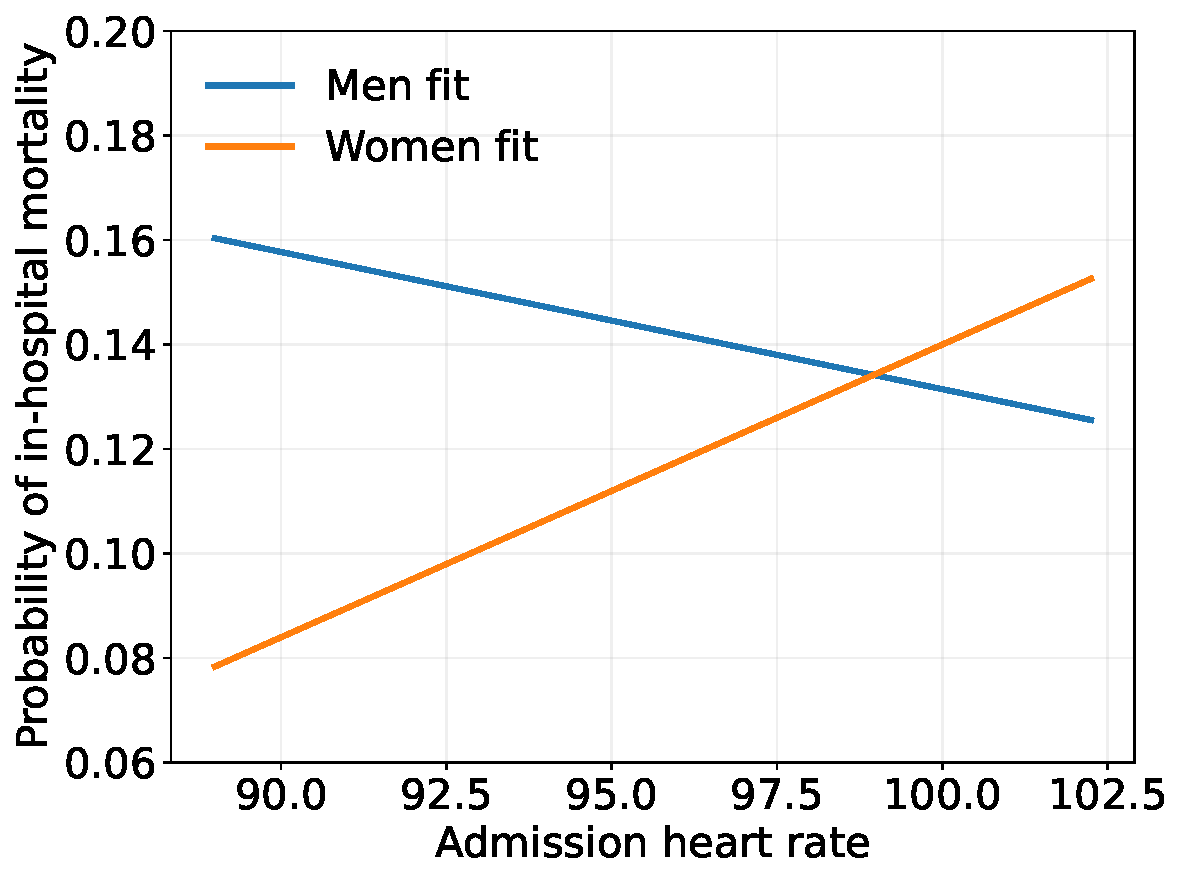
\includegraphics[width=0.75\linewidth]{Sections/Figures/hr_quartile2_mortality_lines.pdf}}
    \caption{Linear probability models of mortality on admission heart rate.}
    \label{fig:hr_quartile2}
\end{figure}

The fact that the explained component points in opposite directions can lead to substantially different descriptive conclusions. When the coefficients for women are used, the positive explained term suggests that differences in admission covariates place men at higher mortality risk, which might prompt a practitioner to examine whether factors such as early differences in blood flow and circulation, underlying disease burden, or overall severity at admission differ across gender. When the coefficients for men are used, the explained component becomes negative. This means that, under men’s own mortality model, the observed covariate differences would predict lower mortality for men relative to women rather than higher. In other words, the same covariates would now be interpreted as offering men a slight mortality advantage. Such sensitivity to the choice of reference rule raises concerns: a descriptive tool that produces contradictory interpretations under equally valid specifications may not offer a stable basis for guiding clinical inquiry.